% Author: Dr. Matthias Jung, DL9MJ
% Year: 2021
\documentclass[convert = false, border=5pt]{standalone}
\usepackage{fontspec}
\setmainfont{Roboto}
\usepackage[siunitx, straightvoltages, europeanresistors, european inductor]{circuitikzgit}
\usepackage{tikz}


\usetikzlibrary{calc, positioning}
\usepackage[siunitx, straightvoltages]{circuitikzgit}
\usepackage{pgfplotstable}
\usepackage{amsmath}
\usepackage{unicode-math}
\setmathfont{Fira Math}
\setmathfont[range=up]{Roboto}
\setmathfont[range=it]{Roboto-Italic}
\setmathfont[range=\int]{Fira Math}
\usepackage[euler]{textgreek}

\begin{document}
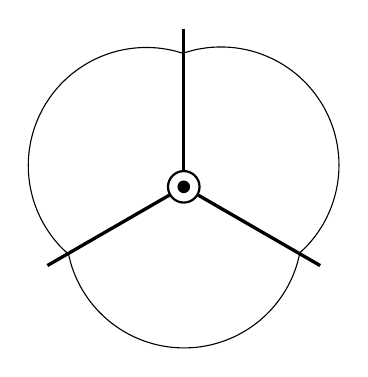
\begin{tikzpicture}
    \foreach\i in {1,2,3}
    {
      \begin{scope}[rotate=120*\i-150]
        \draw[very thick] (0,0) -- (0:2);
        %\draw (0,0) -- (2,0) -- (60:4) -- (120:2);
        %\draw (60:0.5) circle (1.5);
        \begin{scope}[shift={(0.27,0.475)}]
            \draw [smooth,domain=-19:139] plot ({1.5*cos(\x)}, {1.5*sin(\x)});
        \end{scope}
      \end{scope}
    }
    \draw[thick,fill=white] (0,0) circle (2mm);
    \fill                   (0,0) circle (0.8mm);
\end{tikzpicture}
\end{document}
